%!TEX root = main.tex


Fingerprints are ridge and valley patterns presented on the surface of human fingertips.
%
Fingerprints recognition techniques are applied in many areas such as authentication, suspects identification and privacy protection.
%
Typically, to query a fingerprint, the system needs to search and match thousands of fingerprints that are stored in the database. This is a time-consuming process due to huge amount of computation.
%
To mitigate this problem, we can first classify a fingerprint into a basic type and then perform fingerprint match within fingerprints of that type.
%

%
Most of fingerprint classification problems adopts Galton– Henry classification scheme.\cite{henry1905classification} which divide fingerprints into five groups: arch, left Loop, right Loop, tented arch and whorl. 
%
Because arch and tented arch only accounts for a small portion(around 6\%) in human, in some automatic fingerprint identification system, they combine these two classes into one class. 
%
Fig.\ref{fig.fingerprint_classes} shows the five classes of fingerprints. We can see that tented and tented arch are similar.

\begin{figure}[!ht]
	\begin{center}
		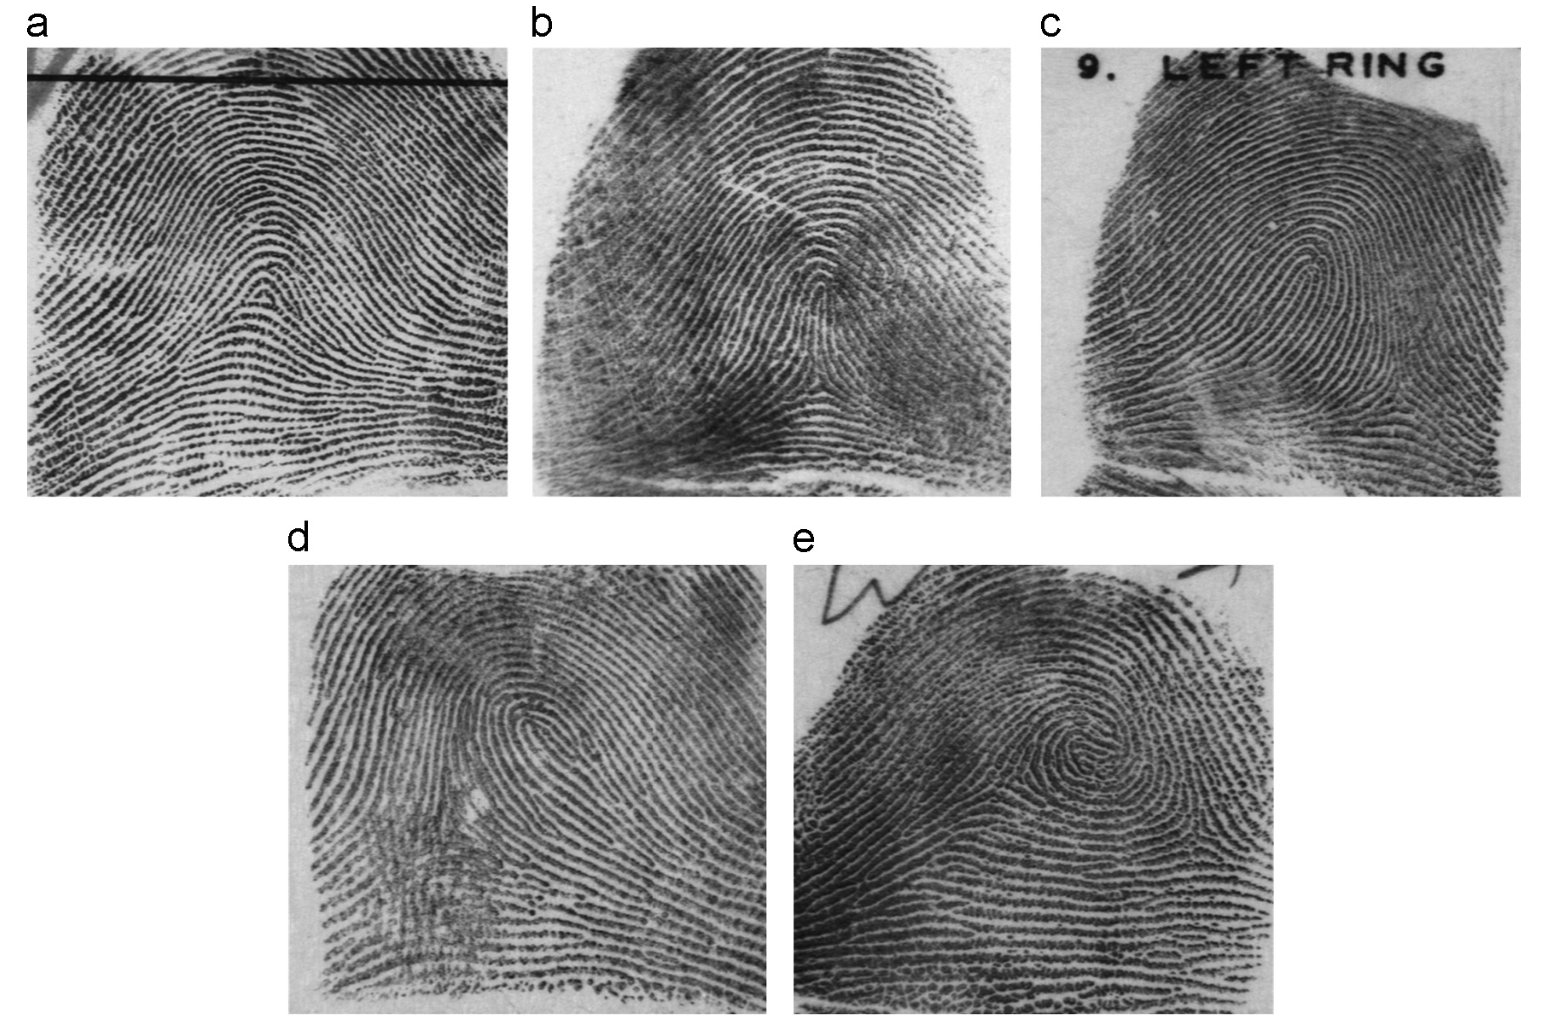
\includegraphics[width=8cm]{fig/Fingerprint_classes.png}
	\end{center}
	\caption{Examples of fingerprint classes: (a) Arch (b) Tented Arch (c) Left Loop (d) Right Loop  (e) Whorl \cite{cao2013fingerprint}} 
	\label{fig.fingerprint_classes}
\end{figure}

